\documentclass[conference]{IEEEtran}
\IEEEoverridecommandlockouts

\usepackage{cite}
\usepackage{amsmath,amssymb,amsfonts}
\usepackage{algorithmic}
\usepackage{graphicx}
\usepackage{textcomp}
\usepackage{xcolor}
\usepackage{booktabs}
\usepackage{array}
\newcolumntype{L}[1]{>{\raggedright\arraybackslash}p{#1}}
\setlength{\emergencystretch}{8em}
\usepackage{tikz}
\usetikzlibrary{positioning,arrows.meta}
% Watermark draf: jadikan komentar tiga baris berikut untuk versi final
\usepackage{eso-pic}
\AddToShipoutPictureBG{\AtPageCenter{\makebox(0,0){\rotatebox{55}{\scalebox{10}{\textcolor[gray]{0.88}{\textsf{DRAFT}}}}}}}
\def\BibTeX{{\rm B\kern-.05em{\sc i\kern-.025em b}\kern-.08em
    T\kern-.1667em\lower.7ex\hbox{E}\kern-.125emX}}
% Label dalam bahasa Indonesia
\renewcommand{\abstractname}{Abstrak}
\renewcommand{\IEEEkeywordsname}{Kata Kunci}
\renewcommand{\tablename}{TABEL}
\renewcommand{\figurename}{Gbr.}
\begin{document}

\title{Deteksi Anomali Kepatuhan pada Data Akademik Pendidikan Tinggi Menggunakan Metode Berbasis Aturan dan Pembelajaran Mesin}

\author{\parbox{\textwidth}{\centering
\parbox[t]{0.45\textwidth}{\centering
{\normalsize 1\textsuperscript{st} Benny Leonard Enrico Panggabean}\\
{\small \textit{Teknik Informatika, Fakultas Teknik} \\
\textit{Universitas Hasanuddin}\\
Makassar, Indonesia \\
bendo01@gmail.com \\
ORCID: 0000-0001-6805-6463}}\hfill
\parbox[t]{0.45\textwidth}{\centering
{\normalsize 2\textsuperscript{nd} Amil Ahmad Ilham}\\
{\small \textit{Teknik Informatika, Fakultas Teknik} \\
\textit{Universitas Hasanuddin}\\
Makassar, Indonesia \\
amil@unhas.ac.id \\
ORCID: 0000-0002-4755-6415}}\\[2ex]
\parbox[t]{0.45\textwidth}{\centering
{\normalsize 3\textsuperscript{rd} Novy N. R. A. Mokobombang}\\
{\small \textit{Teknik Informatika, Fakultas Teknik} \\
\textit{Universitas Hasanuddin}\\
Makassar, Indonesia \\
novy@unhas.ac.id \\
ORCID: 0000-0001-5706-939X}}
}}

\maketitle

\begin{abstract}
Perguruan tinggi di Indonesia melaporkan data akademiknya ke pangkalan data nasional PDDIKTI, dan rekaman yang melanggar aturan pelaporan melemahkan penjaminan mutu dan akreditasi. Makalah ini mengkaji deteksi anomali kepatuhan hanya pada data PDDIKTI, tanpa sistem sumber institusi. Aturan validasi eksplisit yang diambil dari panduan pengguna Feeder PDDIKTI dikombinasikan dengan tiga detektor pencilan tanpa pengawasan: Isolation Forest, Local Outlier Factor, dan autoencoder. Data berasal dari satu institusi dengan tiga program studi dan mencakup 15 semester, termasuk 3.948 rekaman mahasiswa-semester, 348 mata kuliah, dan 1.636 aktivitas mengajar dosen. Karena data telah lolos validasi Feeder, anomali disisipkan ke dalam salinan data, dan deteksi dievaluasi pada 10 penyisipan acak. Aturan mendeteksi pelanggaran eksplisit secara tepat tetapi melewatkan rekaman yang memenuhi semua ambang batas. Detektor pencilan menemukan kembali sebagian rekaman tersebut, dan kinerjanya bergantung pada entitas: untuk aktivitas mengajar, Isolation Forest dan Local Outlier Factor menemukan sekitar dua pertiganya, sedangkan untuk rekaman mahasiswa-semester detektor terbaik menemukan 39 persen. Detektor gabungan mencapai luas area di bawah kurva ROC sebesar 0,982 untuk rekaman mahasiswa-semester. Hasil ini menunjukkan bahwa deteksi berbasis aturan dan pembelajaran mesin saling melengkapi untuk pemeriksaan kepatuhan data akademik.
\end{abstract}

\begin{IEEEkeywords}
\raggedright
deteksi anomali, kepatuhan regulasi, pendidikan tinggi, PDDIKTI, deteksi pencilan, kualitas data
\end{IEEEkeywords}

\section{Pendahuluan}
Perguruan tinggi di Indonesia diwajibkan melaksanakan penjaminan mutu internal serta melaporkan data dan keluarannya ke pangkalan data pendidikan tinggi nasional, PDDIKTI, paling sedikit satu kali setiap semester \cite{permendikbudristek53_2023}. Regulasi yang berlaku saat ini tetap menjadikan PDDIKTI sebagai sumber data utama penjaminan mutu dan menjadikan setiap institusi bertanggung jawab atas kebenaran dan ketepatan data di dalamnya \cite{permendiktisaintek39_2025}. Institusi mengirimkan data tersebut melalui aplikasi Feeder, yang menerapkan sejumlah aturan validasi sebelum sinkronisasi \cite{feeder_guide}. Akurasi data yang dilaporkan memengaruhi akreditasi, pemantauan kinerja, dan akuntabilitas publik.

Masalah kualitas data pada sistem administrasi telah banyak didokumentasikan: kesalahan masuk melalui entri manual, integrasi sistem, dan interpretasi definisi yang tidak konsisten, serta mahal untuk diperbaiki setelah menyebar \cite{whang2023dataquality,zha2025dcai}. Sebuah studi pada perguruan tinggi di Indonesia yang wajib menyampaikan data ke PDDIKTI juga menelusuri rendahnya kualitas data pada tidak adanya kegiatan manajemen kualitas data \cite{sumadi2021dq}. Dalam pelaporan nasional, satu rekaman yang tidak konsisten dapat mendistorsi rasio seperti rasio dosen terhadap mahasiswa atau masa studi, sehingga institusi memerlukan cara sistematis untuk menemukan rekaman yang mencurigakan sebelum pengiriman.

Validasi berbasis aturan dapat menangkap pelanggaran yang dapat dirumuskan secara tertulis, seperti indeks prestasi kumulatif di atas 4,0 atau beban SKS semester di atas 24. Validasi ini tidak dapat menangkap rekaman yang memenuhi setiap ambang batas tetapi tidak lazim secara kombinasi, dan memerlukan aturan baru untuk setiap jenis kesalahan baru. Deteksi pencilan tanpa pengawasan dapat melengkapi aturan karena tidak memerlukan contoh pelanggaran berlabel, tetapi perilakunya pada data pelaporan akademik masih jarang dikaji secara sistematis.

Makalah ini mengevaluasi deteksi anomali kepatuhan berbasis aturan dan pembelajaran mesin dengan hanya menggunakan data PDDIKTI. Pertanyaan penelitiannya adalah: (1) pelanggaran apa saja yang dapat dideteksi oleh aturan validasi Feeder, (2) seberapa baik detektor tanpa pengawasan menemukan rekaman yang memenuhi semua aturan, dan (3) apakah penggabungan keduanya meningkatkan deteksi. Kontribusi utamanya adalah himpunan aturan yang diturunkan dari panduan Feeder dan dipetakan ke atribut PDDIKTI, protokol evaluasi berdasarkan anomali yang disisipkan, serta perbandingan empiris antara aturan, Isolation Forest, Local Outlier Factor, autoencoder, dan gabungannya.

Bagian selanjutnya dari makalah ini disusun sebagai berikut. Bagian~\ref{sec:data} menjelaskan data dan aturan, Bagian~\ref{sec:method} menjelaskan metode dan evaluasi, Bagian~\ref{sec:results} menyajikan hasil, dan bagian terakhir berisi kesimpulan.

\section{Penelitian Terkait}
\subsection{Deteksi Pencilan}
Deteksi anomali telah banyak disurvei, termasuk pendekatan \textit{deep learning} \cite{pang2021deep} dan pandangan terpadu atas metode \textit{deep} dan \textit{shallow} \cite{ruff2021unifying}. Metode-metode tersebut umumnya dikelompokkan menjadi pendekatan berbasis kepadatan, berbasis isolasi, dan berbasis rekonstruksi. Isolation Forest mengisolasi sebuah rekaman melalui pemisahan acak dan menggunakan panjang lintasan sebagai skor anomali \cite{liu2008iforest}; Extended Isolation Forest mengganti pemisahan yang sejajar sumbu dengan hiperbidang acak untuk menghilangkan bias yang ditimbulkannya pada skor \cite{hariri2021eif}. Local Outlier Factor membandingkan kepadatan lokal sebuah rekaman dengan kepadatan tetangganya, sehingga mampu menemukan pencilan relatif terhadap struktur lokal \cite{breunig2000lof}. Autoencoder belajar merekonstruksi rekaman yang tipikal melalui representasi berdimensi rendah, dan galat rekonstruksi yang besar menandakan anomali \cite{pang2021deep,ruff2021unifying}. Detektor-detektor ini tersedia dalam pustaka yang banyak digunakan \cite{scikit-learn,chen2024pyod2}.

\subsection{Tolok Ukur dan Ansambel}
Tolok ukur berskala besar pada data tabular menunjukkan bahwa tidak ada detektor tanpa pengawasan yang mendominasi: dalam studi ADBench terhadap 30 algoritma pada 57 dataset, tidak ada algoritma tanpa pengawasan yang secara statistik mengungguli yang lain \cite{han2022adbench}. Evaluasi ulang terkini atas detektor klasik dan \textit{deep}, termasuk Isolation Forest dan autoencoder, meninjau kembali apakah metode berbasis pohon dapat menyamai metode \textit{deep} \cite{mehta2024benchmark}, dan detektor tabular yang dapat diinterpretasikan telah diusulkan untuk kondisi ketika auditor harus memahami alasan sebuah penandaan \cite{chang2023diad}. Variabilitas ini memotivasi penggunaan ansambel. Evaluasi ansambel tanpa pengawasan yang heterogen mengkaji bagaimana normalisasi skor detektor memengaruhi penggabungan \cite{kluttermann2023ensembles}, dan metode ansambel terkini menyesuaikan setiap skor menggunakan skor rekaman-rekaman tetangganya \cite{yang2024regional}. Penggabungan dalam makalah ini menggunakan peringkat persentil, yang membuat ketiga skala skor dapat dibandingkan sebelum dirata-ratakan.

\subsection{Kualitas Data dan Pemeriksaan Berbasis Aturan}
Masalah kualitas data merupakan hambatan utama bagi sistem berbasis data, dan penelitian terkini memperlakukan kualitas data sebagai perhatian sentral dari AI berpusat-data \cite{whang2023dataquality,zha2025dcai}. Di pendidikan tinggi Indonesia, aturan validasi eksplisit tetap menjadi alat standar: aplikasi Feeder menerapkan pemeriksaan bawaan \cite{feeder_guide}, dan sebuah analisis pada politeknik statistika yang wajib menyampaikan data ke PDDIKTI mengidentifikasi 243 aturan kualitas data serta matriks penilaian untuk data pendidikan, penelitian, dan pengabdian kepada masyarakat \cite{sumadi2021dq}. Aturan memberikan hasil yang tepat dan dapat dijelaskan, tetapi hanya mencakup jenis pelanggaran yang telah diketahui.

\subsection{Deteksi Anomali pada Data Pendidikan}
Deteksi anomali telah diterapkan pada respons mahasiswa yang menyimpang dalam sistem tutor cerdas dengan beberapa metode tanpa pengawasan \cite{gorgun2022aberrant}, dan ukuran berbasis jarak telah digunakan untuk mendeteksi perubahan mendadak pada rekaman pendidikan \cite{smith2021event}. Sepanjang pengetahuan kami, penelitian yang memperlakukan kepatuhan data pelaporan institusi terhadap regulasi pendidikan tinggi sebagai masalah deteksi anomali masih jarang. Oleh karena itu, studi ini mengevaluasi aturan dan detektor tanpa pengawasan pada data yang sama dan mengukur seberapa besar kontribusi masing-masing.

\section{Data dan Aturan Regulasi}\label{sec:data}
\subsection{Dataset PDDIKTI}
Data direplikasi dari layanan web Feeder PDDIKTI ke dalam penyimpanan relasional, satu tabel untuk setiap entitas Feeder. Tabel~\ref{tab:data} merangkum entitas yang digunakan dalam studi ini.

\begin{table}[htbp]
\caption{Entitas dan Atribut PDDIKTI yang Digunakan}
\begin{center}
\begin{tabular}{L{0.27\columnwidth}L{0.61\columnwidth}}
\toprule
\textbf{Entitas} & \textbf{Atribut yang digunakan} \\
\midrule
Biodata mahasiswa & nama, tempat lahir, tanggal lahir \\
Riwayat pendidikan mahasiswa & jenis pendaftaran, SKS diakui, periode masuk dan keluar, tanggal masuk dan keluar \\
Nilai transfer mahasiswa & SKS mata kuliah diakui, nilai diakui \\
Aktivitas kuliah mahasiswa & IPS, IPK, SKS semester, SKS total, status \\
Mata kuliah & SKS total, SKS tatap muka, praktikum, praktik lapangan, dan simulasi \\
Kelas & kapasitas, jumlah mahasiswa, SKS \\
Aktivitas mengajar dosen & rencana dan realisasi pertemuan, SKS substansi \\
Periode perkuliahan & tanggal awal dan akhir, jumlah minggu pertemuan, target mahasiswa baru dan jumlah daftar ulang \\
\bottomrule
\end{tabular}
\label{tab:data}
\end{center}
\end{table}

Ekstrak data mencakup satu perguruan tinggi dengan tiga program studi dan 15 semester akademik (2020/1 hingga 2026/1). Data tersebut berisi 709 mahasiswa (711 pendaftaran), 3.948 rekaman mahasiswa-semester, 348 mata kuliah, 1.607 kelas, 1.765 aktivitas mengajar oleh 90 dosen, dan 2.880 rekaman nilai transfer.

% TODO: prosedur anonimisasi; pernyataan izin/etika penggunaan data PDDIKTI institusi.
\subsection{Aturan Kepatuhan}
{\raggedright Aturan eksplisit diambil dari validasi bawaan aplikasi Feeder PDDIKTI \cite{feeder_guide}. Tabel~\ref{tab:rules} mencantumkan aturan yang dapat dievaluasi hanya dengan data PDDIKTI.\par}

\begin{table}[htbp]
\caption{Kriteria Validasi Berbasis Aturan dari Panduan Feeder PDDIKTI}
\begin{center}
\begin{tabular}{L{0.2\columnwidth}L{0.68\columnwidth}}
\toprule
\textbf{Entitas} & \textbf{Kondisi pelanggaran} \\
\midrule
Mahasiswa & Periode keluar lebih awal dari periode masuk; tanggal masuk tidak sebelum tanggal lulus; usia di bawah 10 tahun \\
Mahasiswa & Pendaftaran baru dengan SKS diakui $>0$; pendaftaran pindahan atau alih jenjang dengan SKS diakui $=0$, atau $>0$ tanpa nilai transfer \\
Aktivitas mahasiswa & IPK $>4{,}0$; IPS $>4{,}0$; IPK $=0$ sementara IPS $>0$; SKS total dan SKS semester keduanya $0$ padahal terdapat pengambilan mata kuliah \\
Aktivitas mahasiswa & Beban SKS semester $>24$ \\
Mata kuliah & Jumlah SKS tatap muka, praktikum, praktik lapangan, dan simulasi berbeda dari SKS mata kuliah, bernilai $0$, atau SKS mata kuliah $>9$ \\
Aktivitas dosen & Realisasi pertemuan $>18$ \\
Periode perkuliahan & Periode perkuliahan yang tumpang tindih dalam satu program studi \\
Mahasiswa & Rekaman ganda berdasarkan nama, tanggal lahir, dan tempat lahir \\
\bottomrule
\end{tabular}
\label{tab:rules}
\end{center}
\end{table}

{\raggedright Semua aturan dalam Tabel~\ref{tab:rules} terpetakan ke atribut yang tersedia dalam skema replikasi. Empat validasi lain dalam panduan Feeder dikecualikan. Pemeriksaan identitas terhadap catatan sipil (DUKCAPIL) memerlukan sumber eksternal: berdasarkan undang-undang administrasi kependudukan, data kependudukan yang digunakan untuk semua keperluan bersumber dari kementerian yang bertanggung jawab di bidang urusan dalam negeri, yang memberikan hak akses kepada pengguna terdaftar dan melarang penyebarluasan data di luar kewenangannya (Pasal 58 ayat (4) dan Pasal 79 ayat (2)--(3)) \cite{uu24_2013}. Oleh karena itu, data tersebut tidak termasuk dalam replika PDDIKTI. Pemeriksaan konsistensi jenis kelamin mahasiswa tidak dispesifikasikan dalam panduan, sehingga nilai acuannya tidak dapat ditentukan hanya dari data PDDIKTI. Pemeriksaan mahasiswa tanpa pendaftaran merupakan pemeriksaan keberadaan antartabel dan bukan pemeriksaan terhadap nilai suatu rekaman, sedangkan pemeriksaan program studi yang tidak terdapat dalam pengaturan periode menyangkut konfigurasi institusi dan bukan rekaman individual; keduanya berada di luar entitas tingkat rekaman yang dikaji di sini. Eksperimen mencakup tiga entitas yang aturannya dapat langsung dievaluasi: rekaman mahasiswa-semester, mata kuliah, dan aktivitas mengajar dosen (1.636 rekaman dengan rencana dan realisasi pertemuan).\par}

% TODO: konfirmasi aturan mana yang dapat diterapkan pada dataset; tambahkan aturan berbasis regulasi
% (misalnya, beban mengajar dosen) hanya jika field datanya tersedia di PDDIKTI.

\section{Metodologi}\label{sec:method}
Alur kerja terdiri atas tiga tahap: deteksi berbasis aturan, deteksi pencilan dengan pembelajaran mesin, dan evaluasi pada data dengan anomali yang disisipkan.

\begin{figure}[htbp]
\centering
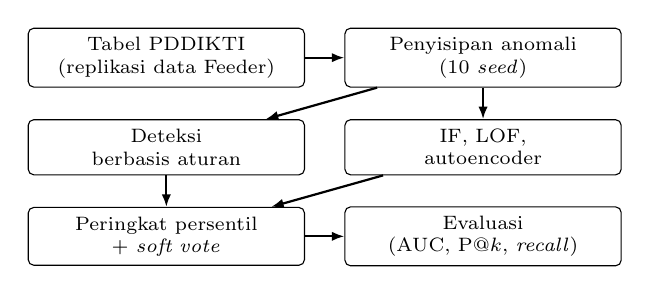
\begin{tikzpicture}[
  node distance=4mm and 5mm,
  box/.style={draw, rounded corners=2pt, align=center, font=\scriptsize, minimum height=7mm, text width=0.27\columnwidth},
  arr/.style={-{Latex[length=1.6mm]}, thick}]
\node[box] (db) {Tabel PDDIKTI\\(replikasi data Feeder)};
\node[box, right=of db] (inj) {Penyisipan anomali\\(10 \textit{seed})};
\node[box, below=of db] (rule) {Deteksi\\berbasis aturan};
\node[box, right=of rule] (ml) {IF, LOF,\\autoencoder};
\node[box, below=of rule] (vote) {Peringkat persentil\\+ \textit{soft vote}};
\node[box, right=of vote] (eval) {Evaluasi\\(AUC, P@$k$, \textit{recall})};
\draw[arr] (db) -- (inj);
\draw[arr] (inj) -- (rule);
\draw[arr] (inj) -- (ml);
\draw[arr] (rule) -- (vote);
\draw[arr] (ml) -- (vote);
\draw[arr] (vote) -- (eval);
\end{tikzpicture}
\caption{Alur deteksi dan evaluasi. Anomali yang disisipkan ditambahkan ke salinan tabel replikasi, lalu aturan dan detektor ML dinilai terhadap label penyisipan.}
\label{fig:pipeline}
\end{figure}

\subsection{Deteksi Berbasis Aturan}
Setiap aturan dalam Tabel~\ref{tab:rules} diimplementasikan sebagai predikat $r_k(x)\in\{0,1\}$ atas rekaman $x$ dari entitas yang bersangkutan. Sebuah rekaman ditandai apabila $\max_k r_k(x)=1$, dan himpunan aturan yang dilanggar disimpan sebagai penjelasan. Aturan dievaluasi per tabel entitas, sehingga tidak diperlukan penggabungan (\textit{join}) dengan sistem eksternal.

\subsection{Deteksi Pencilan dengan Pembelajaran Mesin}
Tiga detektor tanpa pengawasan diterapkan pada fitur numerik yang diturunkan dari tabel yang sama (Tabel~\ref{tab:detectors} merangkum karakteristiknya):
\begin{itemize}
\item \textbf{Isolation Forest}, yang mengisolasi rekaman melalui pemisahan acak sejajar sumbu; rata-rata panjang lintasan yang lebih pendek menandakan rekaman yang lebih anomali.
\item \textbf{Local Outlier Factor (LOF)}, yang membandingkan kepadatan lokal sebuah rekaman dengan kepadatan $k$ tetangga terdekatnya.
\item {\raggedright \textbf{Autoencoder}, jaringan \textit{dense} yang dilatih untuk merekonstruksi rekaman normal; galat rekonstruksi menjadi skor anomali.\par}
\end{itemize}
Fitur dibangun per entitas dari atribut dalam Tabel~\ref{tab:data}. Rekaman mahasiswa-semester menggunakan IPS, IPK, SKS semester, SKS total, dan indikator status aktif. Mata kuliah menggunakan SKS total, keempat komponen SKS, dan selisih antara SKS total dan jumlah komponennya. Aktivitas mengajar menggunakan rencana pertemuan, realisasi pertemuan, dan rasio keduanya. Misalkan $x\in\mathbb{R}^d$ adalah vektor fitur sebuah rekaman. Isolation Forest memberi skor $x$ dengan $s_{\mathrm{IF}}(x)=2^{-E[h(x)]/c(n)}$, dengan $E[h(x)]$ adalah rata-rata panjang lintasan pada seluruh pohon dan $c(n)$ adalah rata-rata panjang lintasan pencarian yang gagal pada pohon biner dengan $n$ titik \cite{liu2008iforest}. LOF memberi skor $x$ dengan rasio rata-rata kepadatan keterjangkauan lokal tetangganya terhadap kepadatannya sendiri, sehingga nilai mendekati 1 berarti normal dan nilai yang lebih besar berarti anomali \cite{breunig2000lof}. Autoencoder memberi skor $x$ dengan kuadrat galat rekonstruksi $s_{\mathrm{AE}}(x)=\lVert x-\hat{x}\rVert_2^2$. Fitur distandardisasi sebelum pelatihan, dan setiap detektor dilatih terpisah untuk setiap entitas pada data tanpa label. Isolation Forest menggunakan 200 pohon, LOF menggunakan $k=20$ tetangga, dan autoencoder berupa \textit{multilayer perceptron} dengan tiga lapisan tersembunyi (berukuran $2d$, $\lfloor d/2\rfloor+1$, dan $2d$ untuk $d$ fitur masukan) yang dilatih paling banyak 400 iterasi; autoencoder diimplementasikan dengan scikit-learn \cite{scikit-learn}.

\begin{table}[htbp]
\caption{Karakteristik Detektor yang Dibandingkan}
\begin{center}
\footnotesize\setlength{\tabcolsep}{3pt}
\begin{tabular}{L{0.17\columnwidth}L{0.2\columnwidth}L{0.25\columnwidth}L{0.25\columnwidth}}
\toprule
\textbf{Detektor} & \textbf{Prinsip} & \textbf{Cocok untuk} & \textbf{Kelemahan} \\
\midrule
Aturan & predikat eksplisit & pelanggaran yang diketahui, tepat dan dapat dijelaskan & melewatkan jenis yang tidak diketahui \\
Isolation Forest & pemisahan acak, panjang lintasan & pencilan global yang terisolasi & lemah terhadap anomali di dalam wilayah padat \\
LOF & rasio kepadatan lokal & penyimpangan lokal, klaster dengan kepadatan berbeda & sensitif terhadap $k$, pencarian tetangga $O(n^2)$ \\
Autoencoder & galat rekonstruksi & kombinasi fitur yang tidak lazim & memerlukan data yang cukup, tidak stabil pada tabel kecil \\
\bottomrule
\end{tabular}
\label{tab:detectors}
\end{center}
\end{table}

\subsection{Evaluasi dengan Anomali yang Disisipkan}
Data yang diekstrak telah lolos validasi Feeder, sehingga hampir tidak ada pelanggaran aturan yang tersisa (Bagian~\ref{sec:data}). Oleh karena itu, \textit{ground truth} dibuat dengan menyisipkan anomali ke dalam salinan data. Untuk setiap aturan dalam Tabel~\ref{tab:rules}, sebagian tetap dari rekaman yang dipilih secara acak dimodifikasi sehingga melanggar aturan tersebut, misalnya menetapkan IPK di atas 4,0, menaikkan SKS semester di atas 24, atau menetapkan periode keluar sebelum periode masuk. Dua kelompok tambahan disisipkan untuk menguji detektor ML di luar aturan eksplisit: rekaman yang tetap berada dalam setiap ambang batas aturan tetapi menyimpang secara kombinasi (misalnya beban SKS tinggi dengan IPK sangat rendah), dan rekaman dengan nilai yang digeser sebesar kelipatan simpangan baku atribut. Rekaman yang disisipi diberi label anomali dan rekaman lainnya diberi label normal. Secara keseluruhan, 5\% rekaman dari setiap entitas disisipi, dibagi rata di antara jenis penyisipan pada entitas tersebut (mahasiswa-semester: empat jenis berbasis aturan dan satu jenis halus; mata kuliah: tiga jenis berbasis aturan; mengajar: satu jenis berbasis aturan dan satu jenis halus). Anomali halus hanya didefinisikan untuk rekaman mahasiswa-semester dan mengajar. Penyisipan diulang dengan 10 \textit{seed} acak.

\subsection{Pengaturan Eksperimen dan Metrik Evaluasi}
Deteksi berbasis aturan dievaluasi dengan presisi, \textit{recall}, dan skor F1 terhadap label penyisipan. Detektor ML dievaluasi dengan luas area di bawah kurva ROC (AUC) dan Precision@$k$, dengan $k$ sama dengan jumlah anomali yang disisipkan. Hasil dilaporkan sebagai rata-rata dan simpangan baku pada 10 penyisipan. Metode berbasis aturan dinilai berdasarkan penanda binernya. Agar ketiga skor ML dapat dibandingkan, masing-masing dikonversi menjadi peringkat persentilnya $\rho_m(x)\in[0,1]$ di dalam tabel entitas, dan skor ML sebuah rekaman adalah rata-rata $\bar{\rho}(x)=\frac{1}{3}\sum_{m}\rho_m(x)$, yaitu \textit{soft vote} tanpa bobot. Detektor gabungan menempatkan rekaman yang ditandai oleh aturan mana pun di peringkat teratas dan mengurutkan sisanya berdasarkan rata-rata peringkat persentil ketiga skor ML; detektor ini menandai sebuah rekaman apabila suatu aturan terpicu atau rekaman tersebut termasuk dalam $k$ rekaman teratas berdasarkan peringkat ML. Precision@$k$ adalah $|\{\text{top-}k\}\cap A|/k$ untuk himpunan $A$ anomali yang disisipkan, dan AUC adalah peluang bahwa anomali yang dipilih secara acak memperoleh skor lebih tinggi daripada rekaman normal yang dipilih secara acak, metrik yang juga digunakan dalam tolok ukur terkini \cite{han2022adbench}. \textit{Recall} himpunan top-$k$ juga dilaporkan secara terpisah untuk anomali berbasis aturan dan anomali halus. Karena anomali yang disisipkan bersifat sintetis, hasilnya mengukur kemampuan deteksi dalam kondisi terkendali, bukan prevalensi pelanggaran yang sebenarnya.


\begin{table}[htbp]
\caption{Pengaturan Eksperimen}
\begin{center}
\begin{tabular}{L{0.34\columnwidth}L{0.54\columnwidth}}
\toprule
\textbf{Butir} & \textbf{Pengaturan} \\
\midrule
Isolation Forest & 200 pohon \\
LOF & $k=20$ tetangga \\
Autoencoder & MLP, lapisan $2d$, $\lfloor d/2\rfloor+1$, $2d$; paling banyak 400 iterasi \\
Prapemrosesan & standardisasi per tabel entitas \\
Penggabungan skor & rata-rata peringkat persentil ketiga skor ML \\
Laju penyisipan & 5\% rekaman per entitas, dibagi rata di antara jenis penyisipan \\
Pengulangan & 10 penyisipan acak \\
Metrik yang dilaporkan & presisi, \textit{recall}, F1 (aturan); AUC, Precision@$k$, \textit{recall} top-$k$ (ML, gabungan) \\
\bottomrule
\end{tabular}
\label{tab:settings}
\end{center}
\end{table}

\subsection{Keterjelasan Temuan}
Sebuah rekaman yang ditandai hanya berguna bagi auditor apabila alasannya terlihat. Untuk deteksi berbasis aturan, penjelasannya adalah himpunan aturan yang dilanggar, yang merujuk langsung ke kriteria dalam Tabel~\ref{tab:rules}. Untuk deteksi ML tidak ada aturan, sehingga penjelasannya berupa vektor fitur rekaman beserta ketiga skor individual dan peringkat persentilnya. Peninjau kemudian dapat melihat, misalnya, bahwa sebuah rekaman tidak lazim bagi autoencoder tetapi tidak bagi Isolation Forest, yang biasanya menunjukkan kombinasi nilai yang tidak lazim alih-alih satu nilai ekstrem. Pembedaan ini berguna karena memberi tahu peninjau apakah perlu mencari satu field yang salah atau ketidakkonsistenan antar-field.

\section{Hasil dan Pembahasan}\label{sec:results}
Tidak ada rekaman dalam data asli yang melanggar aturan mana pun dalam Tabel~\ref{tab:rules} untuk ketiga entitas yang dikaji. Tabel~\ref{tab:auc} melaporkan AUC dan Precision@$k$ pada data dengan anomali yang disisipkan, dan Tabel~\ref{tab:subtle} melaporkan \textit{recall} himpunan top-$k$ menurut jenis anomali.

\begin{table}[htbp]
\caption{AUC dan Precision@$k$ (rata-rata $\pm$ simpangan baku pada 10 penyisipan)}
\begin{center}
\footnotesize\setlength{\tabcolsep}{3pt}
\begin{tabular}{llcc}
\toprule
\textbf{Entitas} & \textbf{Metode} & \textbf{AUC} & \textbf{P@$k$} \\
\midrule
Mahasiswa-semester & Aturan & $0{,}904\pm0{,}004$ & $0{,}810\pm0{,}008$ \\
 & Isolation Forest & $0{,}826\pm0{,}009$ & $0{,}237\pm0{,}044$ \\
 & LOF & $0{,}884\pm0{,}015$ & $0{,}386\pm0{,}029$ \\
 & Autoencoder & $0{,}888\pm0{,}033$ & $0{,}515\pm0{,}058$ \\
 & Gabungan & $0{,}982\pm0{,}006$ & $0{,}823\pm0{,}018$ \\
\midrule
Mata kuliah & Aturan & $1{,}000\pm0{,}000$ & $1{,}000\pm0{,}000$ \\
 & Isolation Forest & $0{,}983\pm0{,}005$ & $0{,}700\pm0{,}092$ \\
 & LOF & $0{,}993\pm0{,}006$ & $0{,}906\pm0{,}027$ \\
 & Autoencoder & $0{,}908\pm0{,}097$ & $0{,}506\pm0{,}173$ \\
 & Gabungan & $1{,}000\pm0{,}000$ & $1{,}000\pm0{,}000$ \\
\midrule
Mengajar & Aturan & $0{,}750\pm0{,}000$ & $0{,}513\pm0{,}016$ \\
 & Isolation Forest & $0{,}979\pm0{,}005$ & $0{,}818\pm0{,}041$ \\
 & LOF & $0{,}865\pm0{,}037$ & $0{,}785\pm0{,}036$ \\
 & Autoencoder & $0{,}872\pm0{,}077$ & $0{,}420\pm0{,}199$ \\
 & Gabungan & $0{,}971\pm0{,}012$ & $0{,}820\pm0{,}043$ \\
\bottomrule
\end{tabular}
\label{tab:auc}
\end{center}
\end{table}

\begin{table}[htbp]
\caption{\textit{Recall} Top-$k$ menurut Jenis Anomali (rata-rata pada 10 penyisipan)}
\begin{center}
\begin{tabular}{llcc}
\toprule
\textbf{Entitas} & \textbf{Metode} & \textbf{Berbasis aturan} & \textbf{Halus} \\
\midrule
Mahasiswa-semester & Aturan & 1{,}000 & 0{,}049 \\
 & Isolation Forest & 0{,}293 & 0{,}015 \\
 & LOF & 0{,}405 & 0{,}308 \\
 & Autoencoder & 0{,}547 & 0{,}390 \\
 & Gabungan & 1{,}000 & 0{,}113 \\
\midrule
Mengajar & Aturan & 1{,}000 & 0{,}027 \\
 & Isolation Forest & 0{,}976 & 0{,}661 \\
 & LOF & 0{,}902 & 0{,}668 \\
 & Autoencoder & 0{,}695 & 0{,}144 \\
 & Gabungan & 1{,}000 & 0{,}639 \\
\bottomrule
\end{tabular}
\label{tab:subtle}
\end{center}
\end{table}

\begin{table}[htbp]
\caption{Presisi, \textit{Recall}, dan Skor F1 Deteksi Berbasis Penanda (rata-rata $\pm$ simpangan baku pada 10 penyisipan)}
\begin{center}
\scriptsize\setlength{\tabcolsep}{2pt}
\begin{tabular}{llccc}
\toprule
\textbf{Entitas} & \textbf{Metode} & \textbf{Presisi} & \textbf{\textit{Recall}} & \textbf{F1} \\
\midrule
Mahasiswa-semester & Aturan & $1{,}000{\pm}0{,}000$ & $0{,}808{\pm}0{,}007$ & $0{,}894{\pm}0{,}004$ \\
 & Gabungan & $0{,}638{\pm}0{,}038$ & $0{,}868{\pm}0{,}033$ & $0{,}735{\pm}0{,}036$ \\
\midrule
Mata kuliah & Aturan & $1{,}000{\pm}0{,}000$ & $1{,}000{\pm}0{,}000$ & $1{,}000{\pm}0{,}000$ \\
 & Gabungan & $0{,}811{\pm}0{,}084$ & $1{,}000{\pm}0{,}000$ & $0{,}894{\pm}0{,}051$ \\
\midrule
Mengajar & Aturan & $1{,}000{\pm}0{,}000$ & $0{,}500{\pm}0{,}000$ & $0{,}667{\pm}0{,}000$ \\
 & Gabungan & $0{,}410{\pm}0{,}146$ & $0{,}854{\pm}0{,}058$ & $0{,}536{\pm}0{,}121$ \\
\bottomrule
\end{tabular}
\label{tab:prf}
\end{center}
\end{table}

Tabel~\ref{tab:prf} melaporkan presisi, \textit{recall}, dan skor F1 untuk dua metode yang menghasilkan penanda biner. Aturan tidak pernah menghasilkan alarm palsu (presisi 1,0), tetapi \textit{recall}-nya dibatasi oleh proporsi anomali halus: 0,808 untuk rekaman mahasiswa-semester dan 0,500 untuk rekaman mengajar. Detektor gabungan menaikkan \textit{recall} menjadi 0,868 dan 0,854 untuk entitas-entitas tersebut, dengan mengorbankan presisi (0,638 dan 0,410), karena detektor ini juga menandai $k$ rekaman teratas berdasarkan peringkat ML, yang sebagian di antaranya normal (sekitar sepertiga untuk rekaman mahasiswa-semester dan sekitar tiga perlima untuk rekaman mengajar). Pada mata kuliah, ketika setiap anomali yang disisipkan melanggar suatu aturan, detektor gabungan mempertahankan \textit{recall} 1,000 tetapi presisinya (0,811) lebih rendah daripada aturan saja.

Secara konstruksi, aturan mendeteksi setiap anomali berbasis aturan yang disisipkan dengan presisi 1,0, karena anomali tersebut dibangkitkan dari aturan yang sama; hal ini bukan bukti akurasi terhadap pelanggaran nyata. Hasil yang informatif menyangkut anomali halus, yang memenuhi setiap aturan. Aturan pada dasarnya tidak menandai satu pun di antaranya; nilai kecil yang tidak nol pada baris aturan dalam Tabel~\ref{tab:subtle} berasal dari skor aturan biner, yang nilai serinya dipecah secara sembarang saat himpunan top-$k$ diisi. Detektor ML menemukan kembali proporsi yang lebih besar, tetapi hasilnya bergantung pada entitas: untuk rekaman mengajar, Isolation Forest dan LOF menemukan sekitar dua pertiga, sedangkan untuk rekaman mahasiswa-semester detektor terbaik, yaitu autoencoder, menemukan 39\%, dan Isolation Forest hampir tidak menemukan sama sekali. Detektor gabungan memberikan AUC terbaik untuk rekaman mahasiswa-semester (0,982) karena aturan menempatkan pelanggaran eksplisit di peringkat teratas, tetapi detektor ini hanya menemukan sedikit anomali halus pada entitas tersebut.

\subsection{Analisis per Entitas}
{\raggedright \textit{Rekaman mahasiswa-semester.} Aturan mencapai AUC 0,904 karena aturan memeringkat penyisipan berbasis aturan (empat perlima dari anomali yang disisipkan) secara sempurna, sedangkan seperlima sisanya yang halus bernilai seri dengan rekaman normal, sehingga menghasilkan $0{,}8+0{,}2\times0{,}5=0{,}9$. Di antara detektor ML, autoencoder adalah yang terbaik pada entitas ini (AUC 0,888, Precision@$k$ 0,515), diikuti oleh LOF (0,884) dan Isolation Forest (0,826). Isolation Forest hanya menemukan 1,5\% anomali halus. Alasan yang masuk akal adalah bahwa rekaman halus, seperti beban SKS tinggi dengan IPK rendah, memiliki nilai yang biasa pada setiap atribut tunggal, sehingga pemisahan acak sejajar sumbu tidak mengisolasinya lebih cepat daripada rekaman normal; detektor yang memperhatikan struktur gabungan bekerja lebih baik. Detektor gabungan menaikkan AUC menjadi 0,982 karena penanda aturan mendorong pelanggaran eksplisit ke peringkat teratas dan peringkat ML mengurutkan sisanya.\par}

\textit{Mata kuliah.} Aturan, dan karenanya juga detektor gabungan, bekerja sempurna pada entitas ini karena semua anomali yang disisipkan berbasis aturan dan masing-masing melanggar kondisi aritmetika pada komponen SKS. LOF adalah detektor ML terkuat (AUC 0,993), dan autoencoder menunjukkan simpangan baku yang besar (0,097) yang konsisten dengan ukuran tabel yang kecil, yaitu 348 rekaman. Entitas ini menggambarkan bahwa aturan yang ditulis untuk batasan aritmetika yang diketahui sulit untuk diungguli, dan bahwa ML memberikan sedikit tambahan ketika batasan yang dilanggar telah dikodekan.

\textit{Aktivitas mengajar.} Pada entitas inilah detektor ML paling berperan. Aturan mencapai AUC 0,750, tetapi Isolation Forest mencapai 0,979 dan detektor gabungan 0,971. Isolation Forest dan LOF menemukan sekitar dua pertiga anomali halus (0,661 dan 0,668), sedangkan autoencoder menemukan 14\%. Rasio realisasi terhadap rencana pertemuan kemungkinan merupakan sinyal berdimensi rendah yang kuat, yang lebih sesuai bagi detektor berbasis isolasi dan kepadatan daripada model rekonstruksi dengan sedikit fitur masukan, meskipun penjelasan ini belum diuji. Detektor gabungan sedikit di bawah Isolation Forest dalam AUC di sini, yang menunjukkan bahwa pemungutan suara tanpa bobot dapat terseret turun oleh anggota yang lebih lemah; bobot yang disetel pada kasus berlabel merupakan perluasan yang wajar.

Hasil ini menunjukkan bahwa deteksi berbasis aturan dan ML saling melengkapi: aturan memberikan deteksi yang tepat dan dapat dijelaskan terhadap pelanggaran eksplisit, dan detektor tanpa pengawasan mencakup penyimpangan yang tidak dijelaskan oleh aturan mana pun. Kesimpulan ini dibatasi oleh kondisi yang terkendali. Anomali halus didefinisikan oleh penulis, data berasal dari satu institusi dengan tiga program studi, dan entitas mata kuliah hanya memiliki 348 rekaman, yang menjelaskan besarnya varians autoencoder. Validasi pada pelanggaran yang terjadi secara alami masih menjadi pekerjaan mendatang.

\subsection{Implikasi Praktis}
Hasil ini menyarankan pembagian kerja dalam alur kerja kepatuhan. Aturan sebaiknya tetap menjadi garis pertahanan pertama karena tepat, murah, dan merujuk kriteria yang berlaku, yang dibutuhkan auditor untuk menindaklanjuti suatu temuan. Detektor tanpa pengawasan paling baik digunakan sebagai tahap kedua yang memeringkat rekaman yang tidak dijelaskan oleh aturan mana pun, sehingga peninjau memeriksa rekaman yang paling tidak lazim terlebih dahulu alih-alih seluruh tabel. Karena detektor-detektor tersebut tidak sepakat mengenai rekaman halus mana yang tidak lazim, terutama untuk data mahasiswa-semester, menampilkan skor detektor individual di samping skor gabungan memberikan informasi lebih banyak kepada peninjau daripada satu angka tunggal. Deteksi juga dapat dijalankan per semester sehingga setiap rekaman dibandingkan dengan rekaman sezamannya dan bukan dengan seluruh riwayat, yang menghindari penandaan rekaman semata-mata karena kondisi akademik berubah dari waktu ke waktu.

\subsection{Ancaman terhadap Validitas}
Tiga keterbatasan memengaruhi sejauh mana hasil dapat digeneralisasi. Pertama, anomali bersifat sintetis: penyisipan berbasis aturan dibangkitkan dari aturan itu sendiri, dan anomali halus mencerminkan asumsi penulis mengenai bentuk rekaman yang tidak konsisten, sehingga angka-angka tersebut menggambarkan kemampuan deteksi dan bukan prevalensi pelanggaran yang sebenarnya. Kedua, data berasal dari satu institusi dengan tiga program studi, dan entitas mata kuliah hanya memiliki 348 rekaman, yang membuat autoencoder tidak stabil. Ketiga, detektor menggunakan hiperparameter bawaan atau yang hanya sedikit disetel; tidak dilakukan pencarian atas jumlah tetangga, jumlah pohon, atau ukuran jaringan, dan pilihan yang berbeda dapat mengubah urutan peringkat antardetektor. Pada data mengajar, 339 dari 1.636 rekaman asli (20,7\%) sudah memiliki realisasi pertemuan nol, dan nilai halus yang disisipkan (paling banyak 3 realisasi pertemuan) tumpang tindih dengan rekaman tersebut; selain itu, 25 dari 410 penyisipan halus (6,1\%) tidak mengubah nilai aslinya. Kedua efek ini membatasi \textit{recall} yang dapat dicapai oleh detektor mana pun pada anomali mengajar yang halus. Perata-rataan pada 10 penyisipan acak mengurangi pengaruh satu pengambilan acak, tetapi tidak menghilangkan bias-bias tersebut.

\section{Kesimpulan}
Makalah ini mengevaluasi deteksi anomali kepatuhan berbasis aturan dan pembelajaran mesin pada data PDDIKTI menggunakan aturan dari panduan validasi Feeder dan anomali yang disisipkan. Aturan mendeteksi pelanggaran eksplisit secara tepat tetapi melewatkan penyimpangan yang memenuhi semua ambang batas, sedangkan Isolation Forest, LOF, dan autoencoder menemukan kembali sebagian penyimpangan tersebut dengan tingkat yang bergantung pada entitas. Detektor gabungan memberikan peringkat keseluruhan terbaik ketika pelanggaran eksplisit dominan, sedangkan pemilihan detektor tanpa pengawasan paling menentukan untuk anomali halus. Pekerjaan mendatang mencakup validasi pada pelanggaran yang terjadi secara alami dan pada institusi lain, entitas lainnya seperti riwayat pendidikan dan periode perkuliahan, penilaian per semester dengan pemungutan suara berbobot yang disetel pada kasus berlabel, serta penautan setiap rekaman yang ditandai dengan teks regulasi yang mungkin dilanggarnya sehingga temuan dapat dijelaskan kepada auditor dalam bahasa alami, misalnya dengan \textit{retrieval-augmented generation} \cite{gao2023rag}.

\section*{Ucapan Terima Kasih}
{\raggedright Penulis mengucapkan terima kasih kepada Institut Teknologi dan Kesehatan Tri Tunas Nasional yang telah menyediakan data PDDIKTI yang digunakan dalam penelitian ini. Penelitian ini tidak menerima pendanaan eksternal.\par}

\begin{thebibliography}{00}
\bibitem{permendikbudristek53_2023} Kementerian Pendidikan, Kebudayaan, Riset, dan Teknologi, ``Peraturan Menteri Pendidikan, Kebudayaan, Riset, dan Teknologi Nomor 53 Tahun 2023 tentang Penjaminan Mutu Pendidikan Tinggi,'' Berita Negara Republik Indonesia Tahun 2023 Nomor 638, Agu. 2023 (dicabut oleh \cite{permendiktisaintek39_2025}).
\bibitem{permendiktisaintek39_2025} \raggedright Kementerian Pendidikan Tinggi, Sains, dan Teknologi, ``Peraturan Menteri Pendidikan Tinggi, Sains, dan Teknologi Nomor 39 Tahun 2025 tentang Penjaminan Mutu Pendidikan Tinggi,'' Berita Negara Republik Indonesia Tahun 2025 Nomor 661, diundangkan 25 Sep. 2025.
\bibitem{uu24_2013} Republik Indonesia, ``Undang-Undang Nomor 24 Tahun 2013 tentang Perubahan atas Undang-Undang Nomor 23 Tahun 2006 tentang Administrasi Kependudukan,'' Lembaran Negara Republik Indonesia Tahun 2013 Nomor 232, Des. 2013.
\bibitem{feeder_guide} Kementerian Pendidikan dan Kebudayaan, ``User guide UI/UX Feeder PDDIKTI, versi 4.0,'' Direktorat Jenderal Pendidikan Tinggi, Des. 2020.
\bibitem{liu2008iforest} F. T. Liu, K. M. Ting, and Z.-H. Zhou, ``Isolation forest,'' in \textit{Proc. 8th IEEE Int. Conf. Data Mining (ICDM)}, 2008, pp. 413--422.
\bibitem{breunig2000lof} M. M. Breunig, H.-P. Kriegel, R. T. Ng, and J. Sander, ``LOF: Identifying density-based local outliers,'' in \textit{Proc. ACM SIGMOD Int. Conf. Management of Data}, 2000, pp. 93--104.
\bibitem{scikit-learn} F. Pedregosa \textit{et al.}, ``Scikit-learn: Machine learning in Python,'' \textit{J. Mach. Learn. Res.}, vol. 12, pp. 2825--2830, 2011.
\bibitem{pang2021deep} G. Pang, C. Shen, L. Cao, and A. van den Hengel, ``Deep learning for anomaly detection: A review,'' \textit{ACM Comput. Surv.}, vol. 54, no. 2, pp. 38:1--38:38, Mar. 2022, doi: 10.1145/3439950.
\bibitem{ruff2021unifying} L. Ruff \textit{et al.}, ``A unifying review of deep and shallow anomaly detection,'' \textit{Proc. IEEE}, vol. 109, no. 5, pp. 756--795, 2021.
\bibitem{hariri2021eif} S. Hariri, M. C. Kind, and R. J. Brunner, ``Extended isolation forest,'' \textit{IEEE Trans. Knowl. Data Eng.}, vol. 33, no. 4, pp. 1479--1489, Apr. 2021, doi: 10.1109/TKDE.2019.2947676.
\bibitem{chen2024pyod2} S. Chen \textit{et al.}, ``PyOD 2: A Python library for outlier detection with LLM-powered model selection,'' arXiv:2412.12154, 2024.
\bibitem{han2022adbench} S. Han, X. Hu, H. Huang, M. Jiang, and Y. Zhao, ``ADBench: Anomaly detection benchmark,'' in \textit{Proc. 36th Conf. Neural Information Processing Systems (NeurIPS), Datasets and Benchmarks Track}, 2022.
\bibitem{mehta2024benchmark} S. Mehta, S. Mehendale, N. Fernandes, J. Sarkar, S. Sarkar, and S. Saha, ``Benchmarking anomaly detection algorithms: Deep learning and beyond,'' arXiv:2402.07281, 2024.
\bibitem{chang2023diad} C.-H. Chang, J. Yoon, S. Arik, M. Udell, and T. Pfister, ``Data-efficient and interpretable tabular anomaly detection,'' in \textit{Proc. 29th ACM SIGKDD Conf. Knowledge Discovery and Data Mining (KDD)}, 2023, pp. 190--201, doi: 10.1145/3580305.3599294.
\bibitem{kluttermann2023ensembles} S. Kl\"uttermann and E. M\"uller, ``Evaluating and comparing heterogeneous ensemble methods for unsupervised anomaly detection,'' in \textit{Proc. Int. Joint Conf. Neural Networks (IJCNN)}, 2023, pp. 1--8, doi: 10.1109/IJCNN54540.2023.10191405.
\bibitem{yang2024regional} J. Yang, S. Rahardja, and S. Rahardja, ``Regional ensemble for improving unsupervised outlier detectors,'' \textit{IEEE Trans. Artif. Intell.}, vol. 5, no. 9, pp. 4391--4402, Sep. 2024, doi: 10.1109/TAI.2024.3381102.
\bibitem{whang2023dataquality} S. E. Whang, Y. Roh, H. Song, and J.-G. Lee, ``Data collection and quality challenges in deep learning: A data-centric AI perspective,'' \textit{VLDB J.}, vol. 32, no. 4, pp. 791--813, 2023, doi: 10.1007/s00778-022-00775-9.
\bibitem{zha2025dcai} D. Zha, Z. P. Bhat, K.-H. Lai, F. Yang, Z. Jiang, S. Zhong, and X. Hu, ``Data-centric artificial intelligence: A survey,'' \textit{ACM Comput. Surv.}, vol. 57, no. 5, pp. 129:1--129:42, May 2025, doi: 10.1145/3711118.
\bibitem{sumadi2021dq} A. R. Sumadi and N. Wilantika, ``Analisis kebutuhan kualitas data dan aturan bisnis data pendidikan,'' \textit{Sistemasi: Jurnal Sistem Informasi}, vol. 10, no. 3, pp. 726--740, Sep. 2021, doi: 10.32520/stmsi.v10i3.1381.
\bibitem{gorgun2022aberrant} G. Gorgun and O. Bulut, ``Identifying aberrant responses in intelligent tutoring systems: An application of anomaly detection methods,'' \textit{Psychol. Test Assess. Model.}, vol. 64, no. 4, pp. 359--384, Dec. 2022.
\bibitem{smith2021event} A. D. Smith, ``Event detection in educational records: An application of big data approaches,'' \textit{Int. J. Bus. Syst. Res.}, vol. 15, no. 3, pp. 271--291, 2021, doi: 10.1504/IJBSR.2021.114936.
\bibitem{gao2023rag} Y. Gao \textit{et al.}, ``Retrieval-augmented generation for large language models: A survey,'' arXiv:2312.10997, 2023.
\end{thebibliography}

\end{document}
